\section{Auswahl des Algorithmus}
\label{sec:Auswahl}
Test

\section{Implementierung in Python}

Nachdem in Kapitel \ref{sec:Auswahl} evaluiert wurde welcher Algorithmus für unsere Problematik am besten angewendet werden kann wurde die Implementierung des \glqq Bees Algorithms\grqq{} in der Programmiersprache Python programmiert.\\\\
Zu Beginn des Programmes musste die Karte mit den dazugehörigen Hindernissen initialisiert werden. Die Karte wurde in Form eines 2D-Koordinatensystems umgesetzt (siehe Abbildung \ref{fig:map_init}).
\begin{figure}[H]
    \begin{tabular}{@{}r@{}} 
        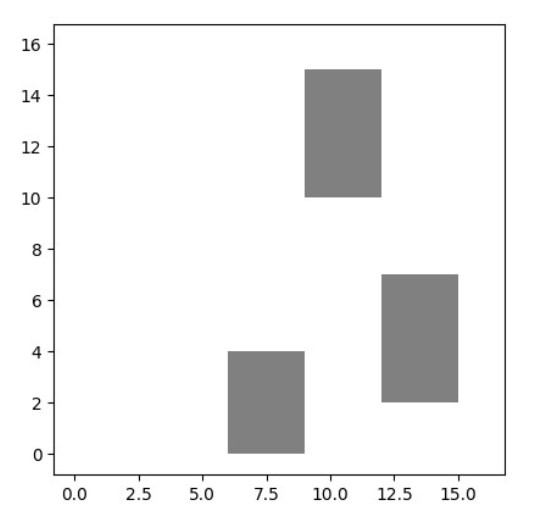
\includegraphics[width=0.5\textwidth, height=0.31\textheight, center]{map_init.jpg}
    \end{tabular}
    \caption{Initialisierte Karte mit Hindernissen\\}   
    \label{fig:map_init}
\end{figure}
Die Menge in der sich der Roboter bewegen darf ergibt sich aus der Gesamtzahl der Karte \emph{K} und den Hindernissen innerhalb der Karte \emph{H}:
\[K\_frei = K - H\]
Als nächstes wird, wie bereits in Kapitel \ref{chap:algorithmen} beschrieben, die Population initialisiert. Für unseren Fall wird der Bienen Algorithmus nicht verwendet um einen optimalen Punkt zu finden, sogar um den optimalen Pfad zu finden. Dabei bildet jede Biene einen Pfad ab. Die Pfade bestehen aus \emph{k} vielen Punkten in Form eines Tuples \emph{(x,y)}. Jeder Pfad wird mit den Koordinaten \emph{(0,0)} initialisiert und muss am Ende am Ziel \emph{(16,16)} ankommen. Die Funktion iteriert von \emph{i = 1} bis \emph{k}, da der erste Punkt des Pfades bereits gesetzt ist:
\begin{figure}[H]
    \begin{lstlisting}[language=python]
def init_population():
    k=7
    i = 1
    path = [(0,0)]
    goal = (16,16)
    while i <= k:
        x = int(random.uniform(0, map_width))
        y = int(random.uniform(0, map_height))
        position = (x,y)
        if is_feasible(position, path[i-1],obstacle_list=obstacle_list):
            path.append((x,y))
            i+=1
        else: 
            x = int(random.uniform(0, map_width))
            y = int(random.uniform(0, map_height))
            position = (x,y)
            
    # Wirf Pfad weg falls das Ziel nach 10 Schritten nicht erreicht ist.
    count = 0
    while not is_feasible(goal,path[i-1],obstacle_list=obstacle_list):
         count += 1
         x = int(random.uniform(0, map_width))
         y = int(random.uniform(0, map_height))
         if is_feasible((x,y), path[i-2], obstacle_list=obstacle_list):
             path[i-1] = (x,y)
         if count > 10:
             return initPopulation()   
    
    path.append(goal)
    return  path
\end{lstlisting}
\caption{Test}
\label{fig:init}
\end{figure} 
Im Quellcode der Abbildung \ref{fig:init} benutzt die stetige Gleichverteilung oder auch uniform distribution function genannt. Die Gleichverteilungsfunktion ist eine Wahrscheinlichkeitsverteilungsfunktion, die angibt, wie wahrscheinlich es ist, dass eine Zufallsvariable einen bestimmten Wert innerhalb eines bestimmten Intervalls annimmt.
Die Gleichverteilungsfunktion ordnet jedem Wert innerhalb des Intervalls die gleiche Wahrscheinlichkeit zu. Das bedeutet, dass jede Zahl innerhalb des Intervalls mit gleicher Wahrscheinlichkeit gezogen wird.\\
Die Formel für die Stetige Gleichverteilung lautet:
\[f(x) = 1/(b-a),\: a \leq x \leq b\]
\[f(x) = 0,\:x < a \:oder\: x > b\]
Dabei ist \emph{a} der untere und \emph{b} der obere Endpunkt des Intervalls. Im Falle dieser Bienen Algorithmus Implementierung wird die Stetige Gleichverteilungsfunktion verwendet, um zufällige Pfadpunkte in den Grenzen der Karte zu erstellen.\\
Nach der Erstellung der Punkte muss überprüft werden, ob der Punkt valide ist. Ein Punkt wird als valide angesehen, wenn die folgenden Bedingungen erfüllt sind:


